The support limits and conditional residual pattern can be localized, but
the available noise controls do not establish a unique, statistically
calibrated physical phase evolution. The most consistent complete-band sign
pattern is localized to the first
night at $\phi=0.376$--$0.393$: the baseline is too faint in the blue band
and too bright in the core and red bands. Earlier blue excess is also present,
but a central depression is not required with the same consistency at every
early phase. This is a conditional residual pattern in the processed data;
the uncertainty and reference tests below delimit its interpretation.

\begin{center}
\small
\begin{tabular}{lrrrr}
\toprule
Actual complete B/C/R phase support & Exposures & Blue & Core & Red\\
 & & \multicolumn{3}{c}{Residual ppm: primary / alternate pixels}\\
\midrule
$0.3043$--$0.3245$ & 14 & $+456/+596$ & $+57/+42$ & $+150/+86$\\
$0.3261$--$0.3498$ & 16 & $+425/+366$ & $+477/-130$ & $+224/+294$\\
$0.3513$--$0.3746$ & 16 & $+307/-9$ & $-788/-88$ & $-340/+19$\\
$0.3761$--$0.3932$ & 12 & $+591/+402$ & $-585/-449$ & $-216/-223$\\
\bottomrule
\end{tabular}
\end{center}
All four rows use the same fully supported exposures for B/C/R, both orders,
and the full-data reference and conditional GP. The two pixel selections
are correlated sensitivities, not independent confirmations or error bars.
The core at $0.326$--$0.350$ and the apparent large feature at
$0.351$--$0.375$ depend strongly on pixel selection. The coarse
$0.35$--$0.40$ bin retains the sign pattern but reduces its amplitude in
the alternate pixels. Thus a precise onset phase or a universal deep trough
is not established by selecting the strongest small bin.

Complete blue coverage ends at $\phi=0.39322$ in the first night and is
absent throughout the second night. Complete core coverage ends at
$\phi=0.41873$ across the two nights; red remains measurable to
$\phi=0.43425$. In particular, the earlier audit's small late blue residual
describes only a shrinking observed portion of the band. It cannot establish
agreement of the complete blue peak with the model. The last declared phase
bin has no complete blue or core measurement.

The late core residual estimates differ substantially between nights.
Both nights retain ten complete-core exposures in a common phase window,
whose limits are $0.40320$ and $0.41806$:
\begin{center}
\small
\begin{tabular}{lrrr}
\toprule
Pixel selection & August 8 core residual & August 20 core residual & Night 2 $-$ night 1\\
 & \multicolumn{3}{c}{ppm}\\
\midrule
Primary & $-41$ & $-977$ & $-936$\\
Alternate & $-87$ & $-845$ & $-758$\\
\bottomrule
\end{tabular}
\end{center}
This difference survives matching the window and exposure counts. The actual
cadences, references and conditional nuisance histories remain different.
It therefore is not an absolute intrinsic night-to-night flux measurement.
The conditional uncertainty of the night difference is about 438 ppm in
either pixel selection; empirical time-block sensitivities span 446--723
and 389--679 ppm. Their two-standard-deviation proxy envelopes include zero.
A reproducible phase-only deficit, or a calibrated detection of intrinsic
night variability, is not established. Stellar/reduction variation and
the inadequacy of the current nuisance model remain possible contributors.

At $\phi=0.376$--$0.393$, the same-exposure blue-minus-core residual is
$1176/852$ ppm in the primary/alternate pixels. Its conditional standard
deviation under the current fixed GP family is $355/345$ ppm, retaining
blue/core covariance. The fixed-planet empirical time-block sensitivity
instead spans $544$--$1052$ and $386$--$901$ ppm. Those large block estimates
include the possible physical residual pattern itself, so they are not proof
that the feature is noise. They demonstrate that these short segments cannot
independently calibrate a robust significance. Some variance estimates are
dominated by approximately one effective block.

No individual fine-bin B/C/R residual, or same-band difference between the
fine primary-product phase bins, keeps its sign in every displayed
two-standard-deviation block-proxy interval. In particular, the red residual
in the candidate interval is only $-216/-223$ ppm with conditional errors
$213/210$ ppm. A separate required red suppression is not established.
Residual ranges across 64 saved noise draws, including separately reprofiled
RV/amplitude, and changes in the local-refit covariance are smaller than these
block sensitivities. The local-refit proxy intervals retain the fixed baseline
center; they are a covariance sensitivity, not a newly optimized phase profile.
These controls do not resolve the uncertainty about omitted time/spectral
systematics.

The native phase-band correction fit has 17 observed columns and full rank
in its chosen rectangular basis; the last blue column is unobserved and
excluded. The complete-band displays retain only 12 or 15 independent rows,
depending on whether common or band-specific exposure support is required.
They cannot reconstruct all 17 corrections. For example, a positive blue
perturbation in one phase bin can cause a negative core response in the next
after the shared reference and GP are fitted. The finite recovery tests pass,
but they do not make the physical interpretation unique.


\begin{figure}[ht]
\centering
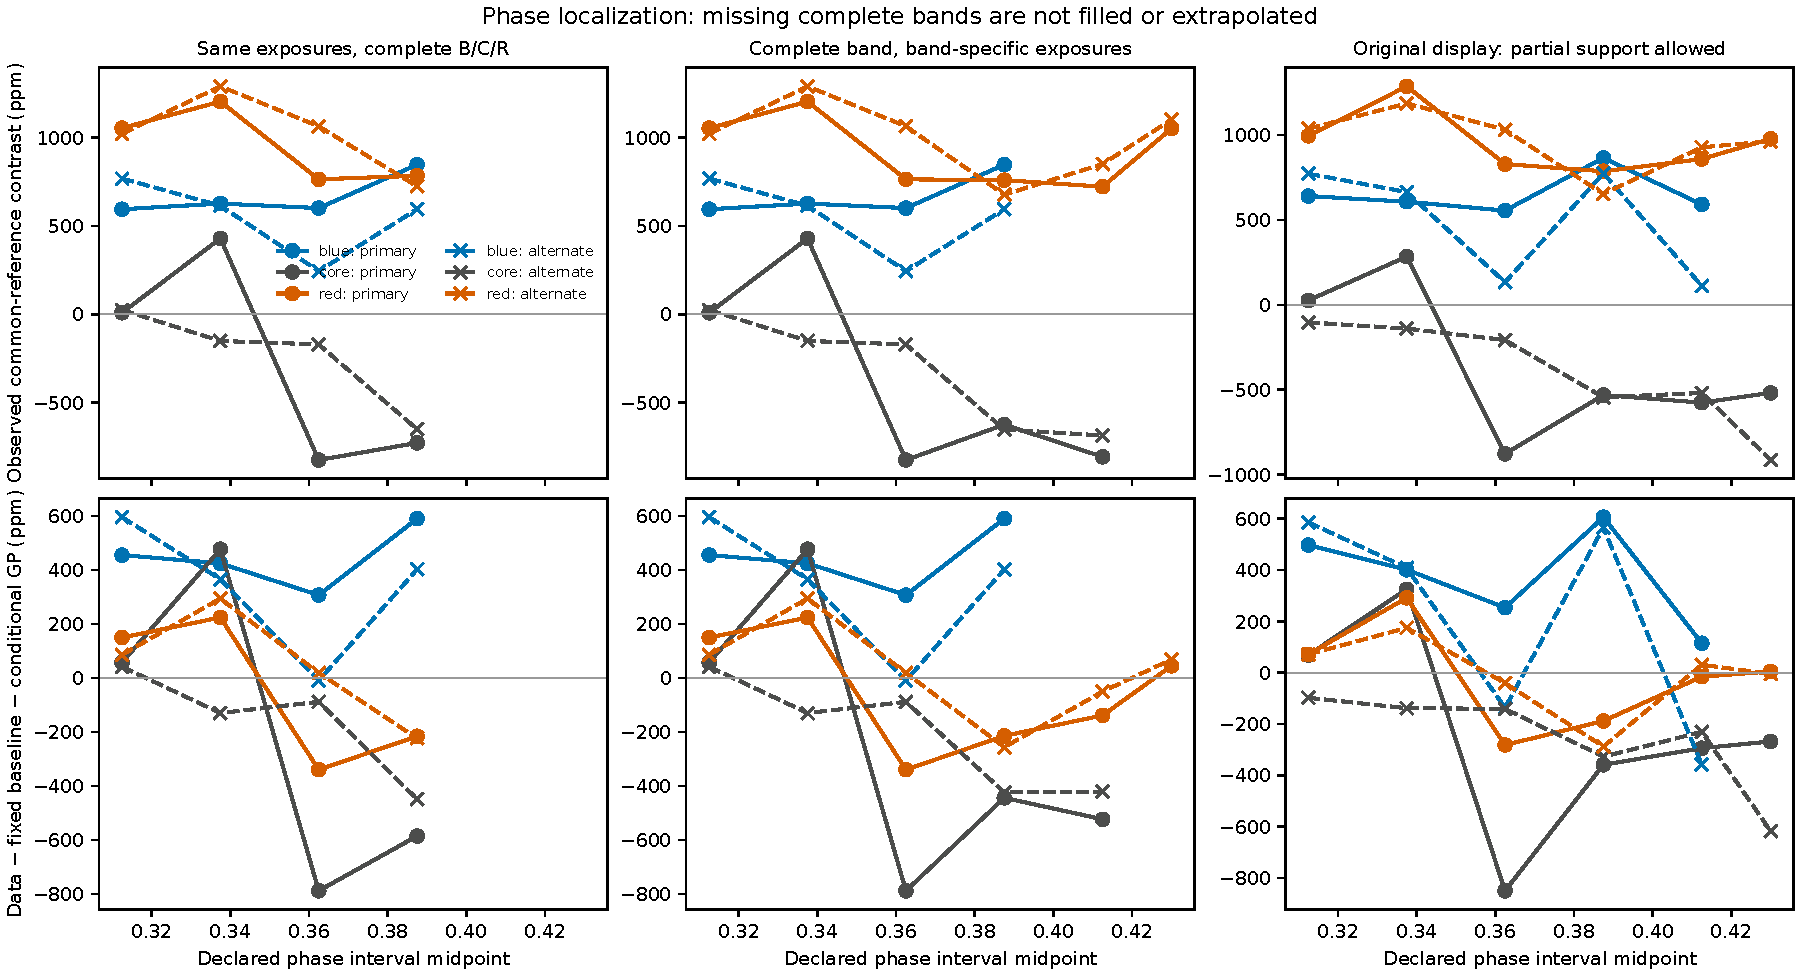
\includegraphics[width=\linewidth]{../mceg/evidence/halpha_phase_localization_20261127/localization/phase_residuals.pdf}
\caption{Complete same-exposure bands (left), complete band-specific support
(middle), and the older partially supported display (right). Solid/dashed
curves are complementary pixel selections, not uncertainty intervals.
Missing complete bands are blank; the x coordinate labels the declared
interval midpoint rather than implying coverage of the whole interval.}
\end{figure}

The practical target for further physical comparison is the complete
$0.376$--$0.393$ blue/core contrast, with its uncertainty and first-night-only
scope retained. The late second-night core requires a separate nuisance and
night-consistency check. An improvement in these selected displays would
still need to be tested on the complete native data; none of these cuts is
adopted as a replacement likelihood.
